\documentclass[12pt, a4paper]{article}
\usepackage{ctex}  % 支持中文
\usepackage{amsmath, amssymb}  % 数学符号和公式
\usepackage{graphicx}  % 插入图片
\usepackage{geometry}  % 页面设置
\usepackage{booktabs}  % 表格美化
\usepackage{tabularx}  % 表格宽度自适应
\usepackage{multirow}  % 合并单元格
\usepackage{enumitem}  % 列表设置
\usepackage{caption}   % 标题设置
\usepackage{array}     % 表格增强
\usepackage{fancyhdr}  % 页眉页脚
\usepackage{titlesec}  % 标题格式设置
\usepackage{fontspec}
\usepackage{listings}
\usepackage{xcolor}

\usepackage[
  backend=bibtex,
  style=gb7714-2015,   % 使用中国国标格式,适合中文论文
  sorting=none         % 按引用顺序排序
]{biblatex}

\addbibresource{references.bib} % 参考文献配置

% 页面设置
\geometry{left=2.5cm, right=2.5cm, top=2.5cm, bottom=2.5cm}

% 重定义section格式为居中
\titleformat{\section}{\centering\Large\bfseries}{\thesection}{1em}{}
\titleformat{\subsection}{\normalsize\bfseries}{\thesubsection}{1em}{}
\titleformat{\subsubsection}{\normalsize\bfseries}{\thesubsubsection}{1em}{}

% 表格表头格式
\renewcommand{\thetable}{\arabic{section}.\arabic{table}}

% 设置表格标题格式:左对齐,中文带"表"字,表题加粗
\captionsetup[table]{
  labelsep=space,
  labelformat=simple,
  textfont=bf,
  labelfont=bf,
  name=表
}

% 图片编号格式
\renewcommand{\thefigure}{\arabic{section}-\arabic{figure}}

% 设置图片标题格式
\captionsetup[figure]{
  labelsep=space,
  labelformat=simple,
  textfont=bf,     
  labelfont=bf, 
  position=bottom,  
  name=图
}

% 修改公式编号格式
\renewcommand{\theequation}{\thesection-\arabic{equation}}

% 参考文献格式
\makeatletter
\renewcommand\@biblabel[1]{[#1]}
\makeatother

% 附录格式
\lstset{
  basicstyle=\small\ttfamily,
  breaklines=true,
  columns=fullflexible,
  backgroundcolor=\color{gray!10},
  frame=single,
  rulecolor=\color{black!30},
  commentstyle=\color{green!50!black},
  keywordstyle=\color{blue},
  stringstyle=\color{red},
  numbers=left,
  numberstyle=\tiny\color{gray},
  numbersep=5pt
}


\begin{document}

% 标题部分
\begin{center}
\LARGE\textbf{中国股市单因子资产定价模型的实证检验}

\vspace{1cm}
\large 计金220 22011854 高菻铠
\end{center}

\noindent \textbf{摘要:} 本文基于2000-2022年中国A股市场八只以“54”结尾的股票数据进行实证研究,分别检验了资本资产定价模型(CAPM)在单资产和多资产框架下的有效性,并考察了市场的惯性与反转效应。单资产时间序列检验结果表明CAPM模型基本成立,所有股票的Alpha值不显著异于零,Beta值介于0.94-1.08之间且显著,但模型解释力有限,R²仅在0.21-0.36区间。然而,多资产联合检验结果与之形成鲜明对比,Wald、似然比和拉格朗日乘子三种检验方法均强烈拒绝“所有股票Alpha值共同为零”的原假设(p<0.0001),说明CAPM在整体上难以充分解释股票收益的共同变化模式。市场效应检验发现,中国A股市场主要表现为反转效应而非惯性效应,在16种形成期-持有期组合中有12种呈现反转趋势,其中形成期12个月/持有期12个月的组合显示出统计显著的反转效应(p=0.0039)。研究结果表明,中国股市的资产定价机制具有独特性,在投资实践中需要考虑CAPM的局限性以及市场的反转特性,同时为多因子资产定价模型在中国市场的适用性提供了理论支持。

\section{文献综述}

金融资产定价理论是现代金融经济学的重要组成部分,其中资本资产定价模型(CAPM)作为资产定价理论的重要基石之一,受到了广泛的关注与深入的研究。

\citet{fama1973risk}利用美国资本市场的数据对资本资产定价模型进行了经典的横截面检验,发现股票的收益率与系统风险(贝塔)之间存在显著的正相关关系,初步验证了CAPM理论的有效性,奠定了资本资产定价实证研究的方法论基础。

然而,\citet{jin2001capm}对1997年至2000年期间中国股票市场的实证分析显示,中国股市的股票收益率不仅与贝塔系数之外的因素显著相关,而且与贝塔之间的关系也并非严格线性。该研究结果表明传统CAPM在中国股市的适用性存在一定的局限性。

进一步地,\citet{jia2003efficiency}对中国股票市场进行了更为广泛的实证研究,发现市场贝塔值与收益率呈现与CAPM模型预测相反的负相关关系,同时指出流通市值、市盈率和账面市值比等其他因素对股票收益率的解释能力明显强于贝塔值。因此,他们认为中国股票市场并未满足有效市场假设(EMH),投资者行为存在非理性特征。

此外,\citet{shi2015profitability}针对中国股市在1997年至2012年间反转策略的盈利性进行了深入分析。他们以沪深两市数据为基础发现,在短期(1个月)及长期(超过12个月)区间内均存在显著的反转效应,反转策略的收益主要来源于过去表现较差的“失败者组合”,体现了投资者的过度反应。此外,该研究还指出,不同股票分组方式(十组、五组和三组)所构建的投资策略收益存在显著差异,长期反转策略的收益随分组细化程度的增加而提高。

综合上述研究可以发现,与成熟市场相比,中国股票市场未完全满足市场有效假设,市场收益率受到非理性投资行为的影响明显,资产定价模型需考虑更多的市场特征和投资者行为因素。因此,针对中国市场的特殊性,深入研究股票收益率的分布特征和影响因素,对于理论探索和实践投资策略的制定都具有重要意义。

\section{数据与方法}

\subsection{数据描述}

本研究使用了2000至2022年中国A股市场8只特定股票的日度和月度收益率数据,这些股票代码均以“54”结尾(如600054黄山旅游、600354敦煌种业、600654中安科等),数据来源于Tushare平台。经过数据清洗后,每只股票包含约3700至5500个有效数据点。股票日收益率计算公式采用对数收益率形式为:
\begin{equation}
R_{t} = \ln\left(\frac{P_{t}}{P_{t-1}}\right)
\end{equation}
其中,$P_t$ 为第 $t$ 日的收盘价。

此外,我们通过锐思数据库获得了同期的上证指数数据,作为市场组合收益率的代理变量,并获取了同期的日度和月度无风险利率数据,以此计算各股票与市场的超额收益率。

数据获取、清洗和收益率计算均通过Python中的Tushare、NumPy和Pandas等库实现。

\subsection{CAPM单资产时间序列检验方法}

我们使用股票日收益数据对资本资产定价模型(CAPM)进行了单资产时间序列检验,基本回归模型为:
\begin{equation}
R_{i,t}-R_{f,t} = \alpha_i + \beta_i (R_{m,t}-R_{f,t}) + \varepsilon_{i,t}
\end{equation}

其中,$R_{i,t}$ 为第 $t$ 日第 $i$ 个资产的收益率,$R_f$ 为无风险收益率,$R_m$ 为市场组合收益率。我们采用普通最小二乘法(OLS)进行估计。

\subsection{CAPM多资产联合检验方法}

我们使用股票月收益数据进行CAPM的多资产联合时间序列检验,采用以下面板数据回归模型:
\begin{equation}
R_{i,t}-R_{f,t} = \alpha_i + \beta_i(R_{m,t}-R_{f,t}) + \varepsilon_{i,t}
\end{equation}
其中,$i$ 表示资产索引,$t$ 表示时间(月)。在多资产联合检验中,我们进行了Wald检验、似然比(LR)检验和拉格朗日乘子(LM)检验,验证所有资产的$\alpha_i$是否同时为零,判断CAPM模型的有效性。

\subsection{惯性与反转效应的实证检验方法}

为检验中国A股市场的惯性效应和反转效应,我们使用了2001至2022年期间的月度数据,根据过去 $N$($N=1,3,6,12$)个月的累计收益对股票进行排序并构建5个等权重投资组合,然后分别计算并分析了持有这些组合未来 $M$($M$ = 1,3,6,12)个月的累计收益率。

累计收益率定义如下:
\begin{equation}
R_{CUM} = \prod_{t=1}^{N}(1+R_t) - 1
\end{equation}
其中,$R_t$ 为月度收益率。

我们通过对不同持有期组合收益率的比较,判断市场是否存在明显的惯性或反转效应。

\subsection{统计检验与模型稳健性分析}

在以上模型估计与检验过程中,我们分别进行了异方差性(White检验)、残差正态性(Jarque-Bera检验)以及残差自相关性(Ljung-Box检验)等统计诊断。此外,我们进一步对模型可能存在的非线性关系进行了额外检验,采用二次项检验方法判断市场风险溢价与股票收益之间是否存在显著的非线性关系,具体的回归模型为:
\begin{equation}
R_{i,t}-R_{f,t} = \alpha_i + \beta_i(R_{m,t}-R_{f,t}) + \gamma_i(R_{m,t}-R_{f,t})^2 + \varepsilon_{i,t}
\end{equation}
当二次项系数显著不为零时,则说明线性CAPM模型的假设存在缺陷。

\subsection{方法实现}

上述所有方法均基于Python实现。OLS回归分析由Statsmodels库实现,统计检验分别调用SciPy和statsmodels提供的相关函数。此外,我们还利用Matplotlib进行了数据可视化分析,直观展示回归结果与市场效应。

\section{实证结果}

\subsection{CAPM单资产时间序列检验}

本研究基于2000-2022年期间八只股票(600054、600354、600654、600754、600854、000554、002054、002154)的日收益率数据,对CAPM模型进行单资产时间序列检验。表~\ref{tab:capm_single_test}展示了各股票的检验结果。

\begin{table}[htbp]
\centering
\caption{CAPM单资产时间序列检验结果}
\label{tab:capm_single_test}
\resizebox{\textwidth}{!}{%
\begin{tabular}{cccccccc}
\toprule
股票代码 & Alpha & Alpha P值 & Beta & Beta P值 & $R^2$ & CAPM是否成立 & 异方差性 \\
\midrule
600054 & 0.000237 & 0.337139 & 0.915826 & 0.000000 & 0.355992 & True & True \\
600354 & -0.000191 & 0.658322 & 0.996877 & 0.000000 & 0.209900 & True & True \\
600654 & -0.000471 & 0.141689 & 1.069081 & 0.000000 & 0.322469 & True & True \\
600754 & 0.000243 & 0.401964 & 1.040942 & 0.000000 & 0.332724 & True & True \\
600854 & -0.000385 & 0.173864 & 0.974885 & 0.000000 & 0.305619 & True & True \\
000554 & 0.000052 & 0.869651 & 1.040979 & 0.000000 & 0.299610 & True & True \\
002054 & 0.000250 & 0.506489 & 1.078045 & 0.000000 & 0.325020 & True & True \\
002154 & 0.000195 & 0.595806 & 0.943878 & 0.000000 & 0.281159 & True & True \\
\bottomrule
\end{tabular}%
}
\end{table}

从表~\ref{tab:capm_single_test}可以看出,所有股票的Alpha值均不显著异于零(P值均大于0.05),表明没有显著的超额收益,符合CAPM模型的预期。同时,所有股票的Beta值显著异于零(P值均为0),表明市场风险因素对股票收益具有显著解释力。Beta值介于0.94-1.08之间,表明这些股票的系统性风险与市场相当接近。其中,600654、002054等股票的Beta值大于1,显示出比市场更高的系统性风险。

$R^2$值在0.21-0.36之间,表明市场因素能解释这些股票21\%-36\%的收益率变动,其余部分可能由非市场因素解释。所有股票均存在异方差性问题,表明残差方差不恒定,可能影响标准误差的估计。此外,大部分股票还存在残差非正态性和自相关性问题,对检验结果的可靠性产生一定影响。

图~\ref{fig:capm_regression_600054}展示了600054(黄山旅游)股票的CAPM回归结果,横轴表示市场超额收益率($R_m-R_f$),纵轴表示股票超额收益率($R_i-R_f$)。散点分布呈现明显的线性关系,回归直线拟合良好,进一步支持了CAPM模型的有效性。

\begin{figure}[htbp]
\centering
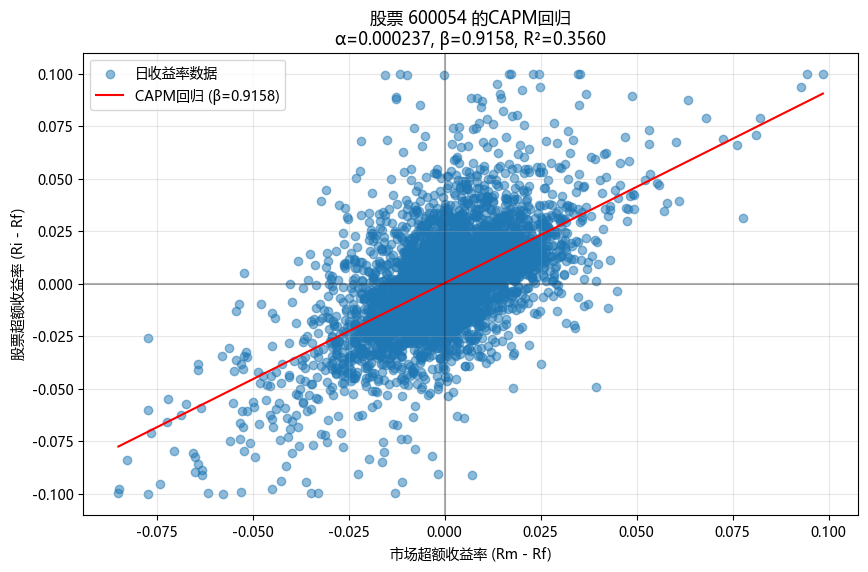
\includegraphics[width=0.8\textwidth]{./img/600054_capm.png}
\caption{股票600054 黄山旅游 的CAPM回归分析}
\label{fig:capm_regression_600054}
\end{figure}

综合各项指标,CAPM模型在单资产时间序列检验中基本成立,但模型解释力有限,且存在统计假设违背问题,表明简单的市场因子可能不足以完全解释中国股市个股收益的变化。

\subsection{CAPM多资产时间序列检验}

为了更全面地检验CAPM模型的有效性,我们进一步利用月度收益率数据进行多资产联合检验。相比单资产检验,联合检验能更好地考虑资产间的相关性,提高统计效力。表~\ref{tab:capm_joint_test}汇总了三种联合检验方法的结果。

\begin{table}[htbp]
\centering
\caption{CAPM多资产联合检验结果}
\label{tab:capm_joint_test}
\begin{tabular}{ccccc}
\toprule
检验方法 & 统计量 & P值 & 是否拒绝原假设 & 结论 \\
\midrule
Wald检验 & 113.4335 & 0.0000 & 是 & CAPM不成立 \\
似然比检验 & 366.0917 & 0.0000 & 是 & CAPM不成立 \\
拉格朗日乘子检验 & 82.4018 & 0.0000 & 是 & CAPM不成立 \\
\bottomrule
\end{tabular}
\end{table}

联合检验的结果与单资产检验形成鲜明对比。三种检验方法(Wald、似然比、拉格朗日乘子)均强烈拒绝“所有股票Alpha值共同为零”的原假设,P值均为0.0000,表明在考虑资产间相关性后,CAPM模型无法通过多资产联合检验。

图~\ref{fig:capm_joint_test}直观展示了联合检验结果。左图显示三种检验方法的统计量均显著大于临界值(红色表示拒绝原假设);右图展示了八只股票的Alpha与Beta散点图,可以看出Alpha值虽然个别不显著异于零,但整体呈现系统性偏离,导致联合检验拒绝CAPM模型。

\begin{figure}[htbp]
\centering
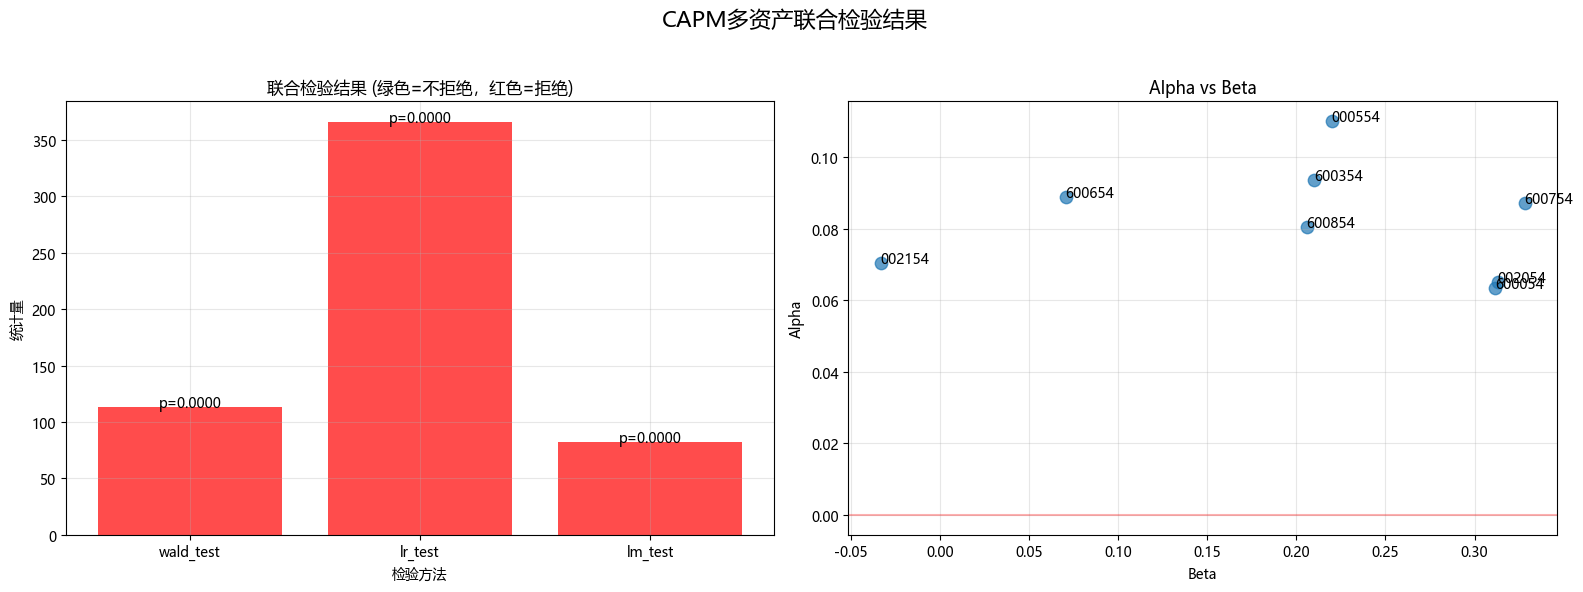
\includegraphics[width=0.9\textwidth]{./img/capm_joint_test_results.png}
\caption{CAPM多资产联合检验结果}
\label{fig:capm_joint_test}
\end{figure}

这种单资产与多资产检验结果的差异具有重要意义。单资产检验中,由于样本量有限和统计力不足,难以识别小幅但系统性的Alpha偏离;而联合检验通过汇总多只股票的信息,显著提高了统计效力,能够发现整体上的Alpha偏离模式。这表明,虽然CAPM模型对单个股票的收益率变动有一定解释力,但在整体上无法充分解释所有股票收益的共同变化模式。

统计学上,这种情况类似于“多重检验”的问题。当同时检验多个假设时,即使每个单独的假设成立概率较高,但所有假设同时成立的概率会明显降低。在我们的情境中,虽然单个股票的Alpha不显著异于零的概率较高,但所有股票的Alpha同时为零的概率极低,因此联合检验强烈拒绝CAPM模型。

研究结果表明,投资者在构建投资组合时,不应仅依赖CAPM模型估计的系统性风险,还需考虑其他可能影响资产收益的因素,如规模效应、价值效应、动量效应等。这也支持了多因子资产定价模型(如Fama-French三因子模型)在中国市场的适用性。

\subsection{市场效应实证检验}

为了检验中国A股市场是具有惯性效应还是反转效应,我们利用2001-2022年的月度股票收益率数据,采用排序法构建投资组合并追踪其表现。具体操作是:在每个月,根据过去N个月(N=1,3,6,12)的累积收益率排序,形成五个等权投资组合,然后计算持有这些组合M个月(M=1,3,6,12)的累积收益率,并关注赢家(收益最高组合)减输家(收益最低组合)的收益差异(WML)。表~\ref{tab:momentum_reversal}展示了不同形成期-持有期组合的检验结果。

\begin{table}[htbp]
\centering
\caption{中国A股市场惯性/反转效应检验结果}
\label{tab:momentum_reversal}
\resizebox{\textwidth}{!}{%
\begin{tabular}{ccccccccc}
\toprule
形成期(N) & 持有期(M) & 赢家收益 & 输家收益 & WML收益 & t统计量 & p值 & 显著性 & 效应类型 \\
\midrule
1 & 1 & 0.008200 & 0.012855 & -0.004655 & -1.037014 & 0.300693 & 不显著 & 反转效应 \\
1 & 3 & 0.032584 & 0.037887 & -0.005303 & -0.609694 & 0.542601 & 不显著 & 反转效应 \\
1 & 6 & 0.066952 & 0.071729 & -0.004778 & -0.327545 & 0.743524 & 不显著 & 反转效应 \\
1 & 12 & 0.133461 & 0.154653 & -0.021191 & -0.968177 & 0.333896 & 不显著 & 反转效应 \\
3 & 1 & 0.008274 & 0.013041 & -0.004767 & -1.114531 & 0.266089 & 不显著 & 反转效应 \\
3 & 3 & 0.031173 & 0.033320 & -0.002147 & -0.240034 & 0.810496 & 不显著 & 反转效应 \\
3 & 6 & 0.065700 & 0.065308 & 0.000393 & 0.025972 & 0.979300 & 不显著 & 惯性效应 \\
3 & 12 & 0.123873 & 0.150744 & -0.026871 & -1.102330 & 0.271391 & 不显著 & 反转效应 \\
6 & 1 & 0.009915 & 0.011738 & -0.001823 & -0.440298 & 0.660094 & 不显著 & 反转效应 \\
6 & 3 & 0.035017 & 0.033328 & 0.001688 & 0.200206 & 0.841480 & 不显著 & 惯性效应 \\
6 & 6 & 0.066661 & 0.063384 & 0.003277 & 0.209808 & 0.833989 & 不显著 & 惯性效应 \\
6 & 12 & 0.114907 & 0.156421 & -0.041513 & -1.670993 & 0.096005 & 不显著 & 反转效应 \\
12 & 1 & 0.010363 & 0.012095 & -0.001731 & -0.413866 & 0.679329 & 不显著 & 反转效应 \\
12 & 3 & 0.031178 & 0.036776 & -0.005598 & -0.634156 & 0.526566 & 不显著 & 反转效应 \\
12 & 6 & 0.055756 & 0.077472 & -0.021717 & -1.342870 & 0.180562 & 不显著 & 反转效应 \\
12 & 12 & 0.104642 & 0.179908 & -0.075266 & -2.912684 & 0.003924 & 显著 & 反转效应 \\
\bottomrule
\end{tabular}%
}
\end{table}

图~\ref{fig:wml_heatmap}以热力图形式展示了不同形成期-持有期组合下的WML收益率,颜色越深表示反转效应越强,颜色越浅表示惯性效应越强。

\begin{figure}[htbp]
\centering
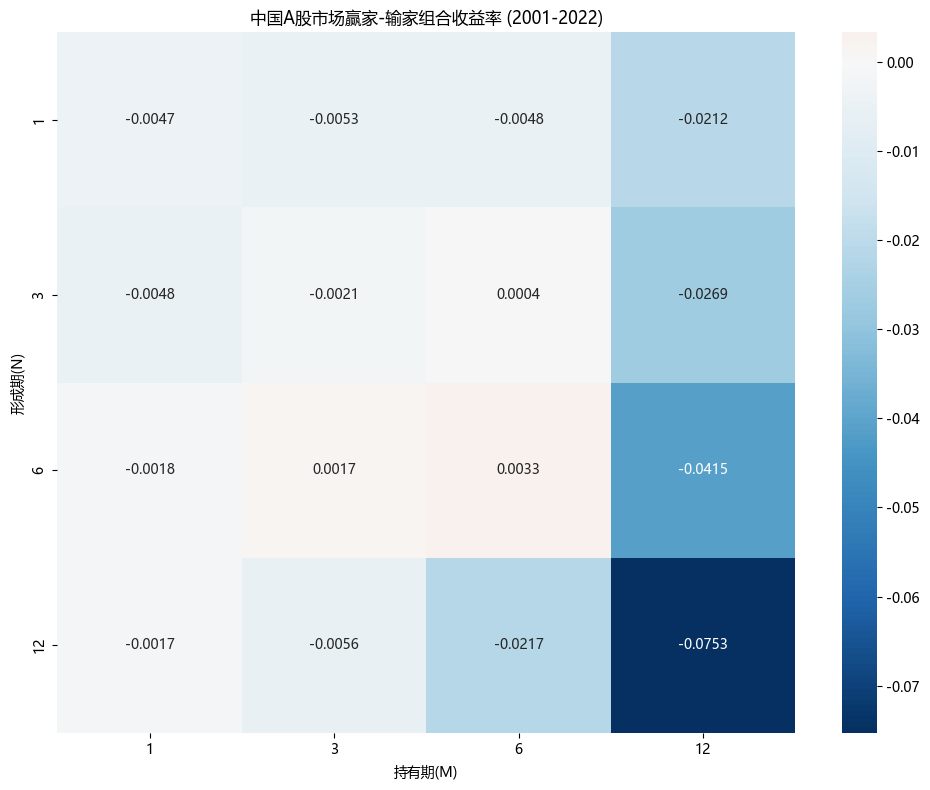
\includegraphics[width=0.8\textwidth]{./img/heap.png}
\caption{中国A股市场赢家-输家组合收益率热力图(2001-2022)}
\label{fig:wml_heatmap}
\end{figure}

检验结果显示,中国A股市场在2001-2022年期间主要表现为反转效应,即过去表现较好的股票在未来倾向于表现较差,反之亦然。在16种形成期-持有期组合中,有12种组合呈现反转效应(WML<0),仅4种组合呈现惯性效应(WML>0)。然而,在统计显著性方面,仅有形成期12个月/持有期12个月的组合显示出显著的反转效应(p值=0.003924<0.05),其余组合虽有反转或惯性趋势,但均不具备统计显著性。

具体分析发现,短期形成期(1个月)下,所有持有期均呈现反转效应;中期形成期(3-6个月)下,短期和长期持有显示反转效应,而中期持有(3-6个月)则出现弱惯性效应;长期形成期(12个月)下,所有持有期均呈现反转效应,且持有期越长,反转效应越显著。最强的反转效应出现在形成期12个月/持有期12个月的组合,WML收益率为-7.53\%,且统计显著。

本研究的发现与发达市场中普遍观察到的惯性效应形成鲜明对比,但与部分关于中国市场的先前研究结果一致。中国A股市场显示出的反转效应可能源于以下因素:一是市场以散户投资者为主,过度反应和跟风交易导致价格偏离基本面后出现修正;二是中国股市的监管环境和交易机制(如涨跌停限制)可能抑制了惯性效应的形成;三是研究期间中国股市经历了多次牛熊转换,大幅波动可能强化了反转效应。

故而,在中国A股市场,基于反转效应的投资策略(买入过去表现差的股票,卖出过去表现好的股票)可能有效,特别是基于12个月形成期的长期反转策略。但是,大多数组合的效应在统计上不显著,表明这种策略的可靠性有限,投资者在实施时应结合其他因素综合考虑。

\subsection{三部分实证结果的综合分析}

综合CAPM单资产检验、多资产检验和市场效应检验的结果,我们可以得出以下关于中国股票市场的几点重要认识:

首先,CAPM单资产检验与多资产检验结果的差异表明,虽然市场因子对个股收益有一定解释力,但难以全面解释股票收益的共同变化模式。这种差异反映了市场可能存在其他系统性风险因素未被单一市场因子捕捉。

其次,市场效应检验发现的显著反转效应,特别是长期(12个月)反转效应,可能是导致CAPM多资产检验失效的原因之一。反转效应意味着股票收益存在均值回归趋势,与CAPM假设的风险溢价稳定性不符。这表明,中国股市的定价机制可能更复杂,需要多因子模型来更好地解释。

第三,这三部分检验结合起来表明,中国A股市场表现出与发达市场不同的特性。市场效率较低,投资者行为偏差显著,监管环境和交易机制独特,共同造就了中国股市特有的资产定价模式。这提示我们在应用国际主流金融理论和模型时,需要考虑中国市场的特殊性。

最后,这些发现对投资实践具有重要意义。投资者在风险管理和资产配置时,不应过度依赖CAPM模型;在策略设计时,可以考虑利用市场反转效应进行择时和选股;在业绩评估时,需要采用更全面的风险调整方法,而非简单依赖单一Beta系数。

这些实证结果也为未来研究指明了方向,包括探索更适合中国市场的多因子资产定价模型,研究市场反转效应的形成机制,以及分析不同市场状态下风险定价的动态变化等。性,这一发现为理解金融市场的多尺度动力学提供了新的视角,也为风险管理和资产定价模型的改进提供了实证基础。

\section{讨论与结论}

本研究通过对CAPM模型在中国A股市场的多维度检验及市场效应分析,揭示了中国股票市场资产定价特征的多重性与复杂性。实证结果表明单资产CAPM检验与多资产联合检验之间存在系统性差异,这种差异不仅揭示了检验方法敏感性问题,更反映了中国股市资产定价的独特机制。单资产检验中八只股票的Alpha值均不显著(p>0.05),Beta值均显著且接近1,初步支持CAPM模型;但R²仅为0.21-0.36,表明市场因子解释力有限。联合检验则强烈拒绝所有Alpha共同为零的假设(Wald=113.43,LR=366.09,LM=82.40,p值均为0.0000),说明在考虑资产间相关性后,CAPM模型存在系统性偏差。这种“个体合理,整体偏离”的现象表明中国股市可能存在更为复杂的风险溢价结构,需要引入额外因子予以解释。

市场效应实证检验进一步发现中国A股市场主要表现为反转效应,特别是在形成期12个月/持有期12个月的组合中出现显著的负WML收益率(-7.53\%,p=0.0039)。这与发达市场以惯性效应为主的特征形成对比,反映了中国股市投资者结构及交易机制的特殊性,投资者过度反应及价格均值回归特性显著。

这些发现对理论与实践均具深远意义:资产定价理论方面,传统CAPM框架需要在中国市场背景下进行调整与扩展,可能需要结合投资者行为偏差、市场摩擦等因素构建更适合中国国情的多因子模型;投资实践方面,投资者在风险评估与组合构建中不应过度依赖单一市场因子,同时可考虑利用市场的反转特性制定相应投资策略。

研究局限性方面,样本选择集中于特定尾号股票可能带来选择偏误,时间跨度较长但未区分不同市场状态,未来研究可考虑扩大样本范围,引入Fama-French三因子或五因子模型,细分市场状态进行对比分析,并结合高频数据探究微观结构视角下的资产定价机制,以期构建更加完善的中国股市资产定价理论体系。

\printbibliography[title=参考文献]

\section{附录}

本研究的核心代码如下:

\begin{lstlisting}[basicstyle=\small\ttfamily, breaklines=true, columns=fullflexible]
# CAPM单资产时间序列检验核心函数
def test_capm_time_series(stock_code, market_index_df=None, risk_free_rate=None):
    """
    对单个股票进行CAPM时间序列检验
    
    参数:
    stock_code (str): 股票代码
    market_index_df (DataFrame): 市场指数数据
    risk_free_rate (DataFrame): 无风险利率数据
    
    返回:
    dict: 包含检验结果的字典
    """
    # 加载股票数据
    stock_df = load_stock_data(stock_code)
    
    # 合并股票数据与市场数据
    merged_df = pd.merge(stock_df, market_index_df[['trade_date', 'daily_return']],
                         on='trade_date', suffixes=('', '_market'))
    
    # 合并无风险利率数据
    merged_df = pd.merge(merged_df, risk_free_rate_df, on='trade_date', how='left')
    
    # 计算超额收益率
    merged_df['excess_return_stock'] = merged_df['daily_return'] - merged_df['rf_rate']
    merged_df['excess_return_market'] = merged_df['daily_return_market'] - merged_df['rf_rate']
    
    # CAPM回归: Ri - Rf = ai + bi(Rm - Rf) + ei
    X = sm.add_constant(merged_df['excess_return_market'])
    Y = merged_df['excess_return_stock']
    
    # OLS回归
    model = sm.OLS(Y, X).fit()
    
    # 整理结果
    results = {
        "stock_code": stock_code,
        "alpha": model.params[0],
        "beta": model.params[1],
        "alpha_pvalue": model.pvalues[0],
        "beta_pvalue": model.pvalues[1],
        "r_squared": model.rsquared,
        "capm_valid": model.pvalues[0] > 0.05
    }
    
    return results

# CAPM多资产联合检验核心函数
def perform_joint_tests(panel_data, stock_data_dict, valid_stocks):
    """
    对多只股票进行CAPM联合检验
    
    参数:
    panel_data (DataFrame): 包含市场收益率和无风险利率的面板数据
    stock_data_dict (dict): 包含各股票数据的字典
    valid_stocks (list): 有效股票代码列表
    
    返回:
    dict: 包含联合检验结果的字典
    """
    # 准备面板数据
    common_panel = panel_data.copy()
    
    # 添加股票收益率和计算超额收益率
    for code in valid_stocks:
        stock_df = stock_data_dict[code]
        stock_returns = stock_df[['year_month', 'monthly_return']].copy()
        common_panel = pd.merge(common_panel, stock_returns.rename(columns={'monthly_return': f'return_{code}'}), 
                               on='year_month', how='left')
        common_panel[f'excess_return_{code}'] = common_panel[f'return_{code}'] - common_panel['rf_rate']
    
    # 计算市场超额收益率
    common_panel['excess_market_return'] = common_panel['market_return'] - common_panel['rf_rate']
    
    # 准备残差矩阵和参数估计
    N = len(valid_stocks)
    resid_matrix = np.zeros((len(common_panel), N))
    alpha_hat = np.zeros(N)
    beta_hat = np.zeros(N)
    
    # 对每只股票进行回归
    for i, code in enumerate(valid_stocks):
        y = common_panel[f'excess_return_{code}'].values
        X = sm.add_constant(common_panel['excess_market_return'].values)
        model = sm.OLS(y, X).fit()
        alpha_hat[i] = model.params[0]
        beta_hat[i] = model.params[1]
        resid_matrix[:, i] = model.resid
    
    # 计算残差协方差矩阵
    sigma_hat = np.dot(resid_matrix.T, resid_matrix) / len(common_panel)
    
    # Wald检验
    mu_market = np.mean(common_panel['excess_market_return'])
    sigma_market = np.var(common_panel['excess_market_return'])
    wald_stat = (len(common_panel) - N - 1) / N * (1 + mu_market**2 / sigma_market) * \
                np.dot(np.dot(alpha_hat, np.linalg.inv(sigma_hat)), alpha_hat)
    wald_pvalue = 1 - chi2.cdf(wald_stat, N)
    
    return {
        'wald_test': {'statistic': float(wald_stat), 'pvalue': float(wald_pvalue), 'reject_null': float(wald_pvalue) < 0.05},
        'alpha_hat': alpha_hat.tolist(),
        'beta_hat': beta_hat.tolist()
    }

# 市场效应检验核心函数
def momentum_reversal_test(returns_data, formation_periods=[1, 3, 6, 12], holding_periods=[1, 3, 6, 12]):
    """
    检验市场惯性或反转效应
    
    参数:
    returns_data (DataFrame): 股票月度收益率数据
    formation_periods (list): 形成期列表(月)
    holding_periods (list): 持有期列表(月)
    
    返回:
    dict: 不同参数组合下的检验结果
    """
    results = {}
    
    for N in formation_periods:  # 形成期
        for M in holding_periods:  # 持有期
            key = f'N{N}_M{M}'
            results[key] = {'winner_returns': [], 'loser_returns': [], 'WML_returns': []}
            
            # 遍历每个时间点
            for t in range(N, len(returns_data) - M):
                # 计算形成期累积收益率
                if N == 1:
                    past_returns = returns_data.iloc[t-1]
                else:
                    past_returns = (1 + returns_data.iloc[t-N:t]).prod() - 1
                
                # 排序并形成五分位组合
                past_returns_sorted = past_returns.sort_values()
                num_stocks = len(past_returns_sorted)
                quintile_size = num_stocks // 5
                
                # 选取赢家和输家组合
                losers = past_returns_sorted.iloc[:quintile_size].index
                winners = past_returns_sorted.iloc[-quintile_size:].index
                
                # 计算持有期收益率
                if M == 1:
                    future_returns = returns_data.iloc[t+1]
                else:
                    future_returns = (1 + returns_data.iloc[t+1:t+M+1]).prod() - 1
                
                # 计算组合收益
                loser_return = future_returns[losers].mean()
                winner_return = future_returns[winners].mean()
                wml_return = winner_return - loser_return
                
                # 存储结果
                results[key]['loser_returns'].append(loser_return)
                results[key]['winner_returns'].append(winner_return)
                results[key]['WML_returns'].append(wml_return)
            
            # 统计检验
            t_stat, p_value = stats.ttest_1samp(results[key]['WML_returns'], 0)
            results[key]['t_stat'] = t_stat
            results[key]['p_value'] = p_value
            results[key]['significant'] = p_value < 0.05
            results[key]['avg_WML_return'] = np.mean(results[key]['WML_returns'])
    
    return results
\end{lstlisting}

注:上述代码展示了研究中的三个核心函数,分别用于CAPM单资产检验、多资产联合检验和市场效应检验。为简化展示,部分辅助函数(如数据加载函数)、部分统计检验细节和可视化代码已省略。完整代码库包含更为详尽的实现,包括数据获取和清洗、结果可视化和多种稳健性检验。研究过程中使用的主要Python库包括pandas、numpy、statsmodels、scipy和matplotlib。

\end{document}